\documentclass[12pt,a4paper,titlepage]{article}
\usepackage[left=2.5cm,text={16cm,20cm},top=4cm]{geometry}
\usepackage[T1]{fontenc}
\usepackage[czech]{babel}
\usepackage[utf8]{inputenc}
% dalsi balicky
\usepackage{graphicx}
\usepackage{enumitem}
\usepackage{indentfirst}
\usepackage{float}
\usepackage{svg}
\usepackage{amsmath}
\usepackage{url}
\usepackage{graphics}
\usepackage{graphicx}
\usepackage{multicol}
\graphicspath{ {images/} }
\usepackage[bookmarksopen,colorlinks,plainpages=false,urlcolor=blue,
unicode,linkcolor=black]{hyperref}

\bibliographystyle{czplain}

%úvodzovky
\providecommand{\uv}[1]{\quotedblbase #1\textquotedblleft}

\begin{document}

\begin{titlepage}
\begin{center}
    {
    	\Huge\textsc{Vysoké učení technické v~Brně}}\\
    \smallskip
    {
    	\huge\textsc{Fakulta informačních technologií}}\\
    \bigskip
    \vspace{\stretch{0.382}} %pomery odpovedajúcí zlatému rezu    
    \huge{Soft computing}\\
    \smallskip
    \Huge{Projekt - fuzzy inference}\\
    \vspace{\stretch{0.618}}
\end{center}
    {\Large \today \hfill David Kozák (xkozak15)  }\\
\end{titlepage}

\newpage

\section{Úvod}
Tento text slouží jako dokumentace mého projektu do předmětu Soft Computing na téma Fuzzy inference. Byla vypracována v rámci zimního semestru akademického roku 2017/2018. První část se zabývá lehkým úvodem do fuzzy množin a fuzzy inference. Zbytek textu slouží jako uživatelská příručka poskytující implementační detaily a také návod, jak s aplikací pracovat.

\section{Fuzzy množiny a fuzzy logika}
Fuzzy množiny jsou zobecněním obyčejných (ostrých) množin, kdy s každým prvkem je spojena hodnota z intervalu <0,1> udávající stupeň příslušnosti (membership degree) prvku z daného univerza
k dané fuzzy množině (nula značí, že prvek v množině určitě není, jednička naopak, že prvek v množině určitě je)\ref{prezentace}. Univerzum může být diskrétní s konečným počtem prvků, diskrétní s nekonečným počtem prvků, či spojité.

Při zavádění fuzzy logiky lze využít fuzzy množiny, kde operace průniku odpovídá AND, sjednocení odpovídá OR a doplněk odpovídá NOT\ref{prezentace}. Existuje mnoho různých definicí fuzzy implikace, v tomto projektu byla využita Mandaniho, která má následující tvar m\textsubscript{a->b} = min(m\textsubscript{A}(a),m\textsubscript{B}(b)).

Fuzzy inference je proces mapování vstupu na výstup s využitím fuzzy logiky. Na počátku je potřeba provést fuzzifikaci vstupních hodnot, poté je možné použít modus ponens, díky kterému se z předpokladů(antecedentů) a faktů vytvoří závěr, opět reprezentovaný fuzzy množinou, kterou lze nyní defuzzifikovat.  Příklad aplikace jednoduchého pravdla typu \textit{if A then B} naleznete na obrázku \ref{oneRuleSimple}, příklad pravidla \textit{if A and B then C} na obrázku \ref{oneRule}, a příklad dvou pravidel na obrázku \ref{twoRules}.


\section{Uživalská příručka}
Tato sekce se zabývá dvěma tématy, implementačními detaily a příkazy pro překlad a spuštění projektu.

\subsection{Ovládání aplikace}
Po spuštění aplikace se objeví hlavní okno, jak můžete vidět na obrázku \ref{emptyWindow}. Po kliknutí na tlačítka Fact X, Atecendent X či Consequent, kde X je přirozené číslo, se zobrazí dialog umožňující nastavit různé funkce příslušnosti. Konkrétně je možné zvolit konstantní, lineární, gausovu (obrázek \ref{setDetailsGaussian}), trojúhelníkovou (obrázek \ref{setDetailsTriangle}) a trapezoid. Pro rychlou demonstraci lze zvolit možnost \textit{Run Demo} v horní liště v kolonce \textit{Help}, která zvolí náhodné fuzzy množiny a demonstruje pravidlo \textit{if a and b then c}.

\begin{figure}[!htbp]
	\centering
	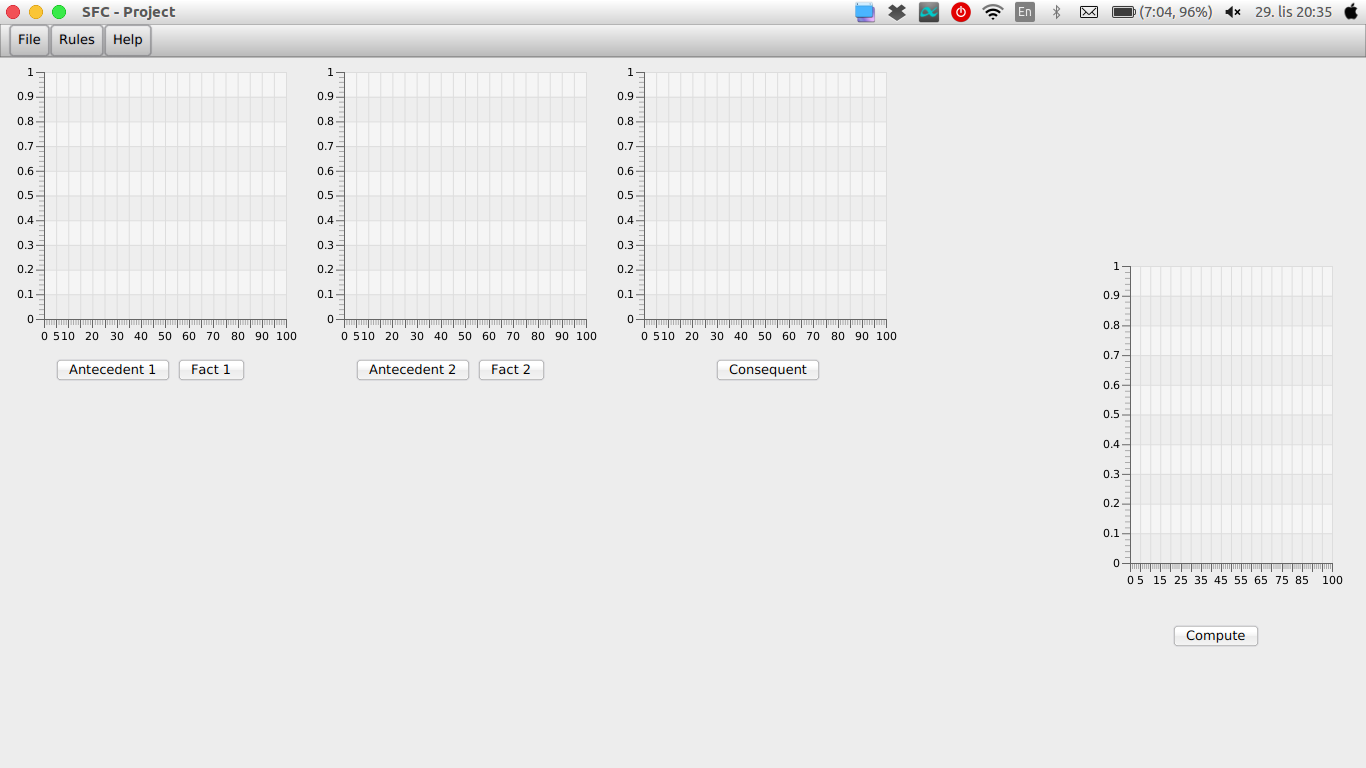
\includegraphics[scale=0.3]{emptyWindow}
	\caption{Vzhled aplikace po otevření}
	\label{emptyWindow}
\end{figure}

\begin{figure}[!htbp]
	\centering
	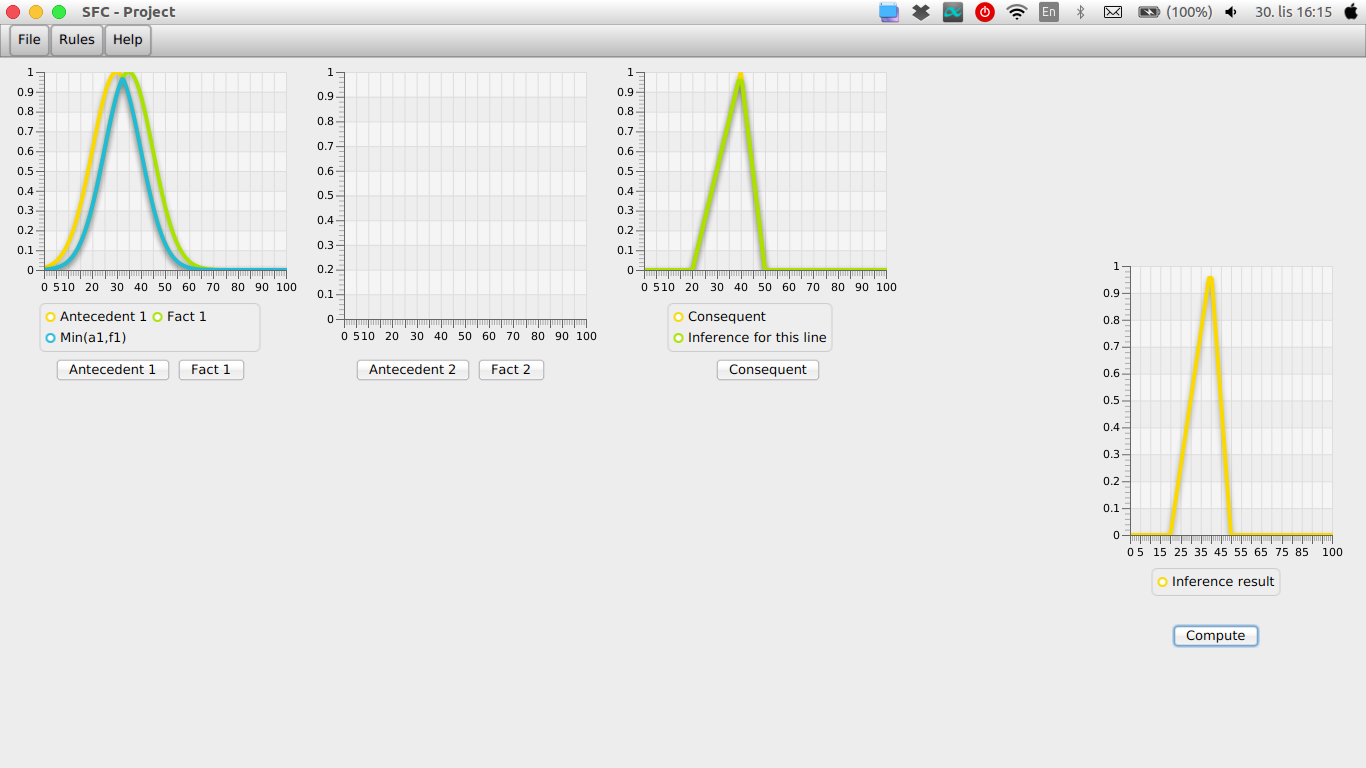
\includegraphics[scale=0.3]{oneRuleSimple}
	\caption{Jedno pravidlo jednoduché}
	\label{oneRuleSimple}
\end{figure}

\begin{figure}[!htbp]
	\centering
	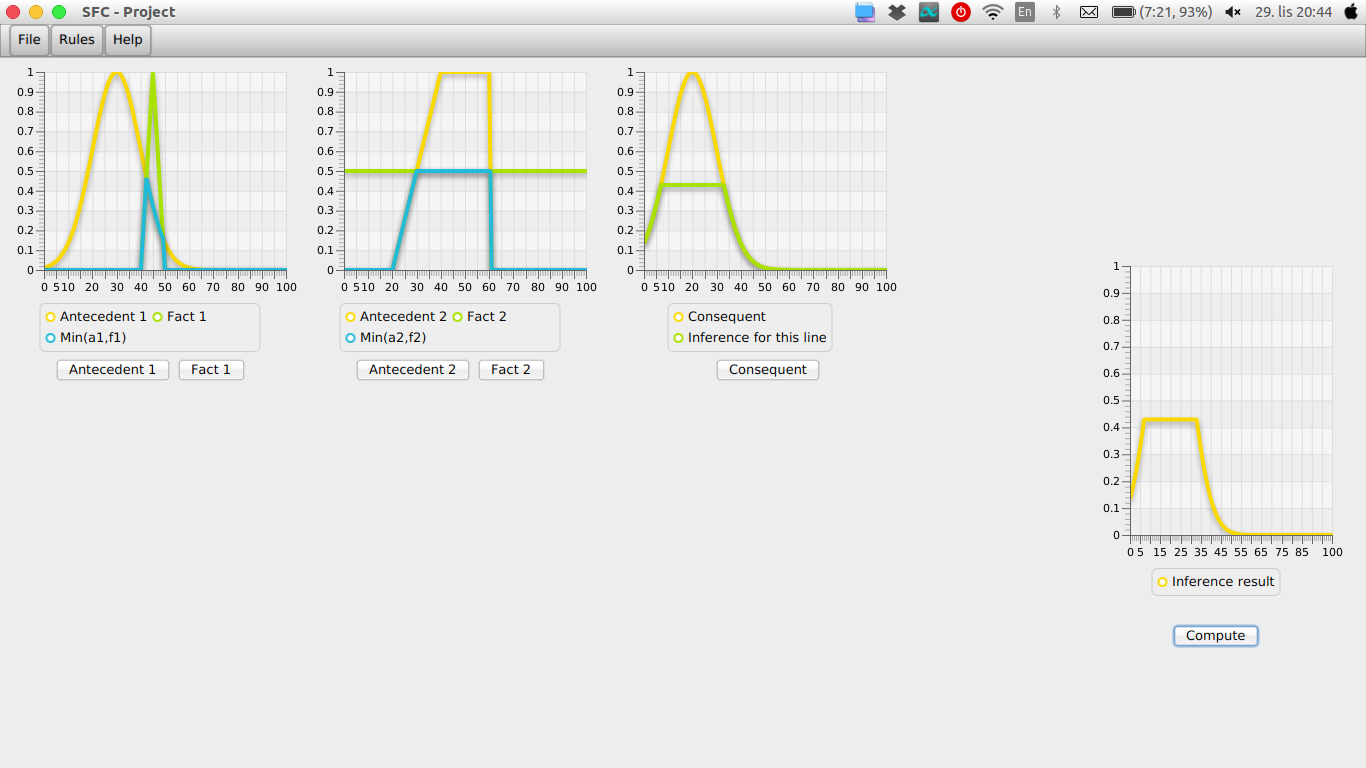
\includegraphics[scale=0.3]{oneRule}
	\caption{Jedno pravidlo}
	\label{oneRule}
\end{figure}

\begin{figure}[!htbp]
	\centering
	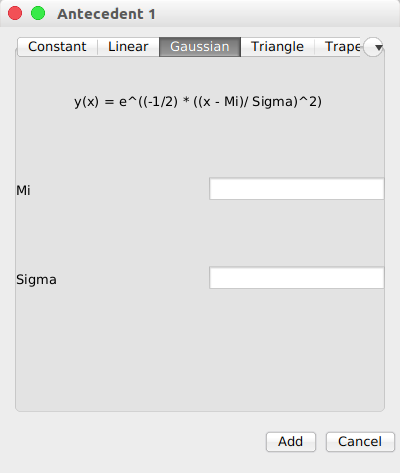
\includegraphics[scale=0.5]{setDetailsGaussian}
	\caption{Detaily gausovské membership funkce}
	\label{setDetailsGaussian}
\end{figure}

\begin{figure}[!htbp]
	\centering
	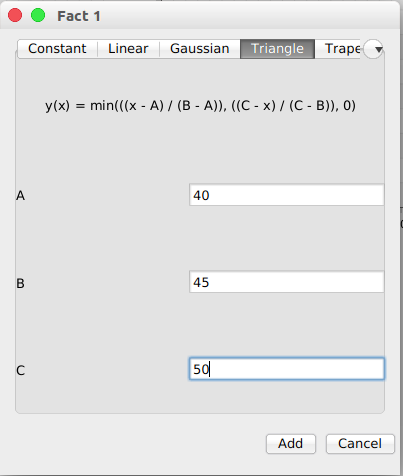
\includegraphics[scale=0.5]{setDetailsTriangle}
	\caption{Detaily trojúhelníkové membership funkce}
	\label{setDetailsTriangle}
\end{figure}

\begin{figure}[!htbp]
	\centering
	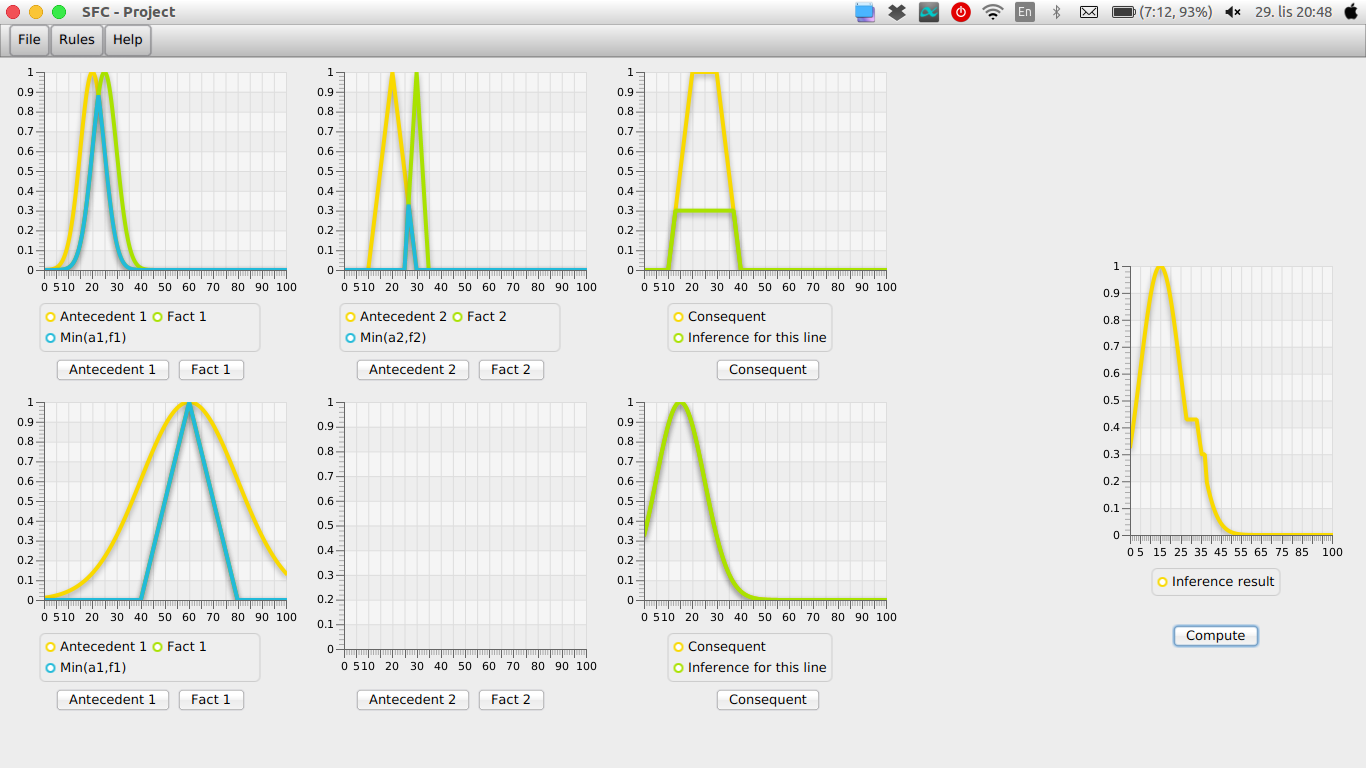
\includegraphics[scale=0.3]{twoRules}
	\caption{Dvě pravidla}
	\label{twoRules}
\end{figure}


\subsection{Implementační detaily}
Projekt byl implementován v programovacím jazyku Java s využitím GUI frameworku JavaFX. Krom toho jsou též využity externí knihovny ProjectLombok, junit, mockito, afterburner.fx a aquafx.

\subsection{Překlad a spuštění}
Projekt lze přeložit s pomocí build skriptu pro ant nebo pomocí maven. Pro jednoduché spuštění na Merlinovi je připraven skript \textit{config.sh}. Jelikož velikost využitých knihoven je větší než 2MB, nejsou v archivu přiloženy, ale skript je stáhne z maven repozitářů. Ke spuštění tohoto skriptu je tedy potřeba přístup k internetu. Výstupem překladu je jar archiv build/dist/fuzzy\_inference.jar. Aplikace samotná lze spustit pomocí skriptu \textit{run.sh}.

Jelikož původní projekt byl vytvořen jako maven projekt, je ho též možno přeložit příkazem \textit{mvn clean install}, tedy za přepokladu, že je maven na daném stroji nainstalovaný.


\section*{Reference}
\begin{enumerate}[label={[\arabic*]}]
\item ZBOŘIL F. Slajdy k přednáškám Soft Computing[Online] \\
     \href{https://www.fit.vutbr.cz/study/courses/SFC/private/17sfc\_9.pdf}
          {https://www.fit.vutbr.cz/study/courses/SFC/private/17sfc\_9.pdf}
     \label{prezentace}
\end{enumerate}
\end{document}